\documentclass[12pt]{article}
\usepackage[margin=1in]{geometry}
\usepackage{enumitem}
\usepackage{titlesec}
\usepackage{parskip}
\usepackage{graphicx}
\usepackage{xcolor}
\usepackage{hyperref}
\usepackage{fontenc}

\title{\textbf{Katz and Mair 1995 RG Notes}\\
\large Katz, Richard S., and Peter Mair. ``Changing Models of Party Organization and Party Democracy: The Emergence of the Cartel Party'' [1995].\\
\textit{Party Politics} 1(1): 5-28.}
\author{}
\date{}

\begin{document}

\maketitle

Emergence of the ``Cartel Party,'' in which ``colluding parties become agents of the state and employ the resources of the state (the party state) to ensure their own collective survival''

The mass party as a single cross-sectional element of party type development throughout modern politics, rather than an end stage which parties will inevitably evolve into (eventually with either stability or overall decay)

\begin{center}

\includegraphics[width=0.85\textwidth]{figure-1.png}
\end{center}

\begin{center}
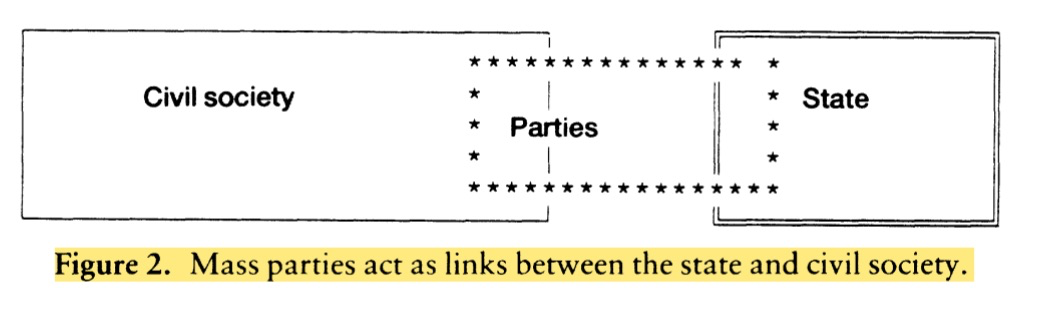
\includegraphics[width=0.85\textwidth]{figure-2.png}
\end{center}

\begin{center}
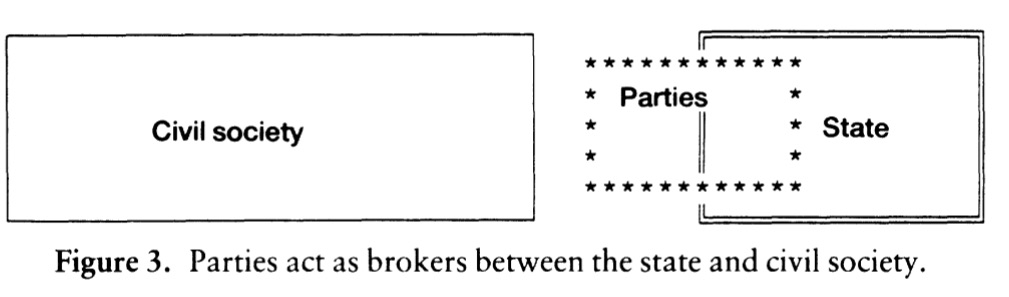
\includegraphics[width=0.85\textwidth]{figure-3.png}
\end{center}

Cartel parties largely act as this third option: parties become somewhat consubstantial with the state, and must make connections to civil society which they do not necessarily organically have

\end{document}
